
%==========================================================================================================
% MULAI BAB III
%==========================================================================================================
\chapter{PERANCANGAN DAN IMPLEMENTASI}
\label{chap:perancangan}
%==========================================================================================================
% subbab
%==========================================================================================================
\section {Deskripsi}
\label{sec:gambaran_aplikasi}
Secara konvensional model suatu objek nyata (misalnya gedung) biasanya disajikan dengan membuat sebuah  miniatur atau maket seperti yang ditunjukkan gambar \ref{fig:real_virtual_ar}.a. Dengan adanya model atau maket tersebut, seseorang bisa dengan mudah melihat atau mengetahui objek yang dimodelkan tersebut secara nyata, akan tetapi pembuatan model atau maket tersebut membutuhkan waktu yang lama serta biaya yang mahal. Dengan menggunakan komputer dan \textit{software} tertentu pemodelan objek bisa disajikan secara virtual seperti terlihat pada gambar \ref{fig:real_virtual_ar}.b. Dengan menggunakan \textit{software}, pemodelan objek memang lebih menghemat biaya serta waktu, namun interaksi dengan dunia nyata sangat kurang. Aplikasi \textit{viewer} model 3D  dengan teknologi \textit{Augmented Reality} yang penulis rancang ini menggabungkan kedua kelebihan pemodelan secara nyata dan \textit{software}, yaitu kemudahan pembuatan model 3D (secara virtual) dan juga interaksi terhadap dunia nyata seperti diilustrasikan pada gambar \ref{fig:real_virtual_ar}.c.

\begin{figure}[h]
\begin{center}
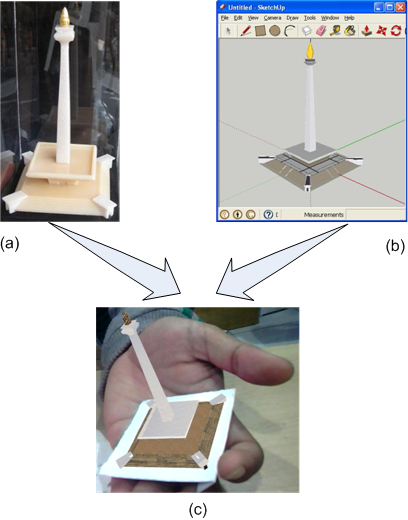
\includegraphics[width=10cm]{./images/real_virtual_ar}
\caption{\label{fig:real_virtual_ar} Gambaran aplikasi \textit{viewer} objek 3D virtual dengan \textit{Augmented Reality}}
\end{center}
\end{figure}

Aplikasi yang dirancang dengan teknologi AR ini, seolah-olah menggabungkan objek virtual dengan objek nyata, dalam hal ini objek nyatanya berupa gambar dengan pola tertentu (disebut \textit{marker}) dan objek virtualnya berupa model 3D. Sistem menggunakan teknik \textit{spatial display} (pembahasan pada subbab \ref{subsec:spatial_display} dengan \textit{screen display} (bisa berupa monitor ataupun proyektor). Secara garis besarnya gambaran sistem dapat dilihat pada gambar \ref{fig:gambaran_sistem_ar}. 
%Kamera yang terhubung ke komputer  menangkap sebuah citra dari \textit{marker} yang berfungsi sebagai \textit{tracker}. Dengan adanya pengenalan pola, sistem akan mengenali gambar tersebut. Setelah pola tersebut terindentifikasi maka sistem akan menampilkan model 3D yang telah ditentukan jika pola tersebut ditemukan. Proses tersebut berlangsung secara \textit{real-time} sehingga objek virtual yang tampil di komputer akan mengikuti pergerakan \textit{tracker}.
\begin{figure}[h]
\begin{center}
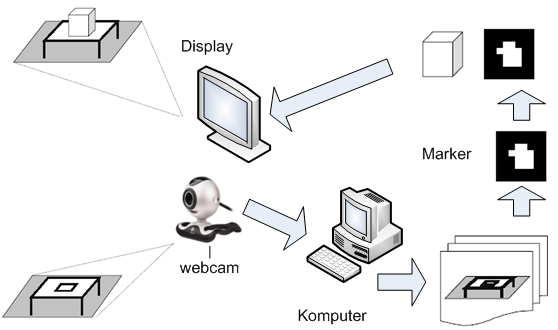
\includegraphics[width=10cm]{./images/gambaran_sistem_ar}
\caption{\label{fig:gambaran_sistem_ar} Gambaran sistem secara umum}
\end{center}
\end{figure}

\textit{webcam} berfungsi sebagai media \textit{visi} bagi aplikasi AR untuk mendapatkan video masukan. Kamera mengambil \textit{frame}-\textit{frame} video untuk dapat diterima oleh komputer. Komputer memproses citra digital yang diakuisisi oleh \textit{webcam}, \textit{frame} demi \textit{frame}. Komputer akan mendeteksi pola yang mirip dengan \textit{marker} dari setiap \textit{frame} video tersebut, yang kemudian lokasi dan rotasi dari \textit{marker} dapat ditentukan. Dengan informasi tersebut, objek \textit{virtual} digabungkan dengan video dari \textit{webcam} dan me-\textit{render}-nya sesuai dengan informasi posisi yang diperoleh dari \textit{marker} tersebut. Dengan demikian, \textit{marker} tersebut seolah-olah berfungsi sebagai \textit{tracker} untuk model 3D virtual. Proses tersebut berlangsung secara \textit{real-time} sehingga model 3D virtual yang tampil di media \textit{display} akan mengikuti pergerakan \textit{tracker}.

%FLARToolKit memiliki kelemahan dalam hal \textit{rendering} model. Sehingga sebuah \textit{library} yang dapat merender model 3D dengan kualitas tinggi seperti Papervison3D diperlukan. Papervision3D akan meload data objek 3D dan menampilkan objek tersebut. Pada aplikasi ini penulis menggunakan objek 3D dengan format collada yang sudah didukung oleh Papervision3D

\section {Perancangan Aplikasi}
\label{sec:desain_aplikasi}
Aplikasi yang dirancang merupakan aplikasi berbasis \textit{web} atau disebut juga \textit{Rich Internet Applications} (RIAs), tujuannya agar mudah diakses dari komputer atau juga \textit{handheld} tanpa perlu instalasi aplikasi. Berdasarkan penjelasan pada subbab \ref{subsec:adobe_flash_platform}, penulis memilih Adobe Flash sebagai \textit{Framework} RIAs dengan SDK (\textit{software Development Kit}) Adobe Flex. Bahasa script yang digunakan adalah ActionScript yang merupakan bahasa pemrograman berorientasi objek. ActionScript mendukung \textit{event-driven programming} (Pemrograman berbasis \textit{event}). \textit{event-driven programming} merupakan paradigma pemrogaman yang alur program ditentukan dari \textit{event}, \textit{input} sensor atau pesan dari program lain. Paradigma ini sangat cocok untuk pengembangan aplikasi ini, dikarenakan aplikasi menerima input dari kamera atau \textit{webcam}.

Aplikasi ini dibangun menggunakan FLARManager, seperti telah dijelaskan pada subbab \ref{subsec:FLARManager}, FLARManager dapat mempermudah dan mempercepat pengembangan aplikasi yang menggunakan \textit{library} FLARToolKit. \textit{Library} FLARToolKit merupakan salah satu \textit{tracking library} AR di lingkungan Flash (subbab \ref{subsec:FLARToolKit}). Di dalam FLARManager sudah termasuk pengaturan kamera untuk masukan video, kelas untuk mengatur pola marker yang digunakan, dan juga kelas untuk memudahkan interaksi dengan \textit{library} engine 3D, dengan demikian aplikasi yang dibangun tidak perlu berhubungan langsung dengan \textit{library} FLARToolKit.

\begin{figure}[h]
\begin{center}
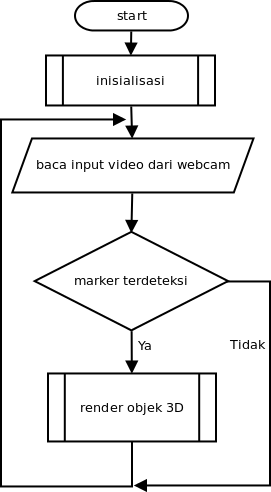
\includegraphics[width=6cm]{./images/flowchart/aplikasi}
\caption{\label{fig:flowchart_aplikasi} Diagram alir aplikasi secara umum}
\end{center}
\end{figure}

Secara keseluruhan, aplikasi dapat digambarkan dengan diagram alir pada gambar \ref{fig:flowchart_aplikasi}. Aplikasi melakukan inisialisasi terlebih dahulu sebelum melakukan \textit{tracking} \textit{marker}, \textit{marker} dideteksi dari masukan video \textit{webcam}, jika \textit{marker} terdeteksi maka objek 3D di-\textit{render}. 

Secara garis besarnya, dalam perancangan aplikasi ini ada tiga bagian utama yaitu sebagai berikut:
\nopagebreak
\begin{itemize}
\item Inisialisasi\\
Inisialisasi semua hal yang diperlukan untuk proses aplikasi (\textit{marker}, objek 3D, engine 3D)
\item \textit{Tracking} \textit{marker}\\
Marker yang digunakan lebih dari satu pola, setiap \textit{marker} dengan pola tertentu akan menjadi \textit{tracker} objek 3D tertentu pula.
\item \textit{Rendering} objek 3D\\
Objek 3D dirender dan diatur posisinya sesuai dengan posisi \textit{marker} yang terdeteksi.
\end{itemize}

Penulis merancang aplikasi ini atas beberapa kelas (gambar \ref{fig:diagram_kelas}), agar memudahkan pengembangan aplikasi. Kelas utama adalah \textbf{AR3DV}, yang mengatur jalannya aplikasi, mulai dari inisialisasi hingga \textit{render} objek 3D. 

\begin{figure}[h]
\begin{center}
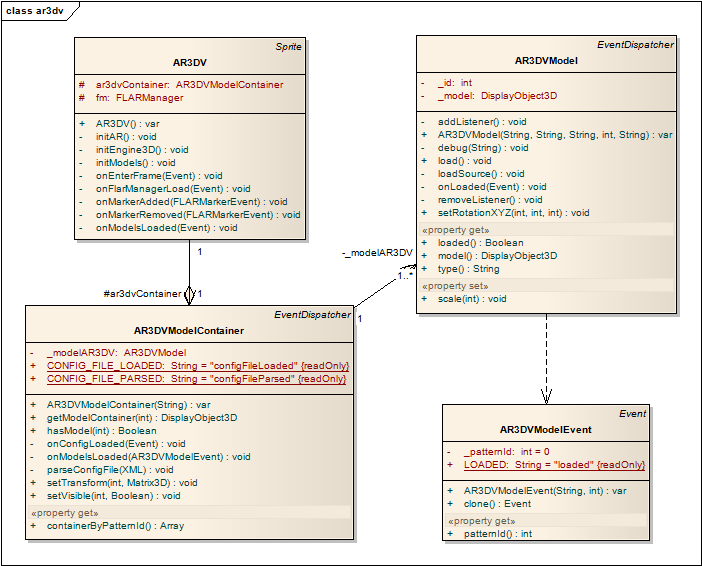
\includegraphics[width=14cm]{./images/class}
\caption{\label{fig:diagram_kelas} Diagram kelas aplikasi}
\end{center}
\end{figure}

Tiga kelas lainnya berhubungan dengan objek 3D dan inisialisasinya, yaitu sebagai berikut:
\begin{itemize}
\item AR3DVModelContainer\\
Kelas yang mengatur objek 3D apa saja yang di-\textit{load}, serta menyediakan objek 3D yang dapat dipanggil dari kelas utama. \textbf{AR3DVModelContainer} menggunakan file konfigurasi dengan format xml untuk model objek 3D yang akan di-\textit{load}.
\item AR3DModel\\
Kelas yang berfungsi untuk me-\textit{load} objek 3D, serta mengatur rotasi dan skala objek.
\item AR3DModelEvent\\
\textit{Loading} model memerlukan waktu yang cukup lama tergantung ukuran \textit{file} objek 3D. Karena itu \textit{load} objek 3D dilakukan secara asinkron. Kelas \textbf{AR3DVModelContainer} akan me-\textit{load} semua \textit{file} objek 3D dengan bantuan kelas \textbf{AR3DModel}. Agar kelas \textbf{AR3DVModelContainer} mengetahui objek 3D tertentu telah di-\textit{load}, diperlukan sebuah pesan yang disebut juga \textbf{Event}. Penulis membuat kelas \textbf{AR3DModelEvent} agar bisa digunakan \textbf{AR3DModel} untuk menyampaikan pesan ke kelas \textbf{AR3DModelContainer}.
\end{itemize}

\subsection{Inisialisasi}
\label{subsec:inisialisasi}
Pada tahap ini ditentukan \textit{marker} yang akan digunakan, sumber input video nya, objek 3D yang akan digunakan serta \textit{engine} 3D yang digunakan untuk me-\textit{render} objek 3D. Pada bagian inisialisasi ini, objek 3D diinisialisasi terlebih dahulu karena \textit{loading} objek 3D memerlukan waktu yang cukup lama. Setelah objek 3D di-\textit{load}, kemudian FLARManager dan \textit{engine} 3D diinisialisasi. Deskripsi inisialisasi digambarkan oleh \textit{sequence diagram} gambar \ref{fig:init_sequence}.

\begin{figure}[h]
\begin{center}
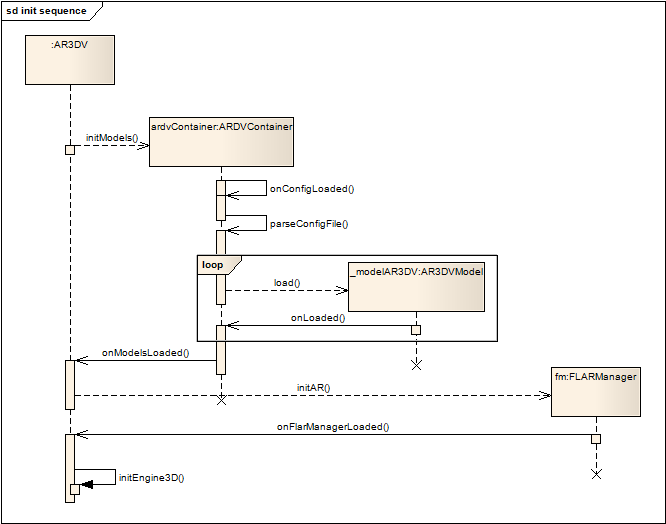
\includegraphics[width=14cm]{./images/init_sequence}
\caption{\label{fig:init_sequence} \textit{Sequence diagram} inisialisasi}
\end{center}
\end{figure}

\subsubsection {Inisialisasi Model 3D}
\label{subsubsec:inisialisasi_model_3d}
Model 3D yang akan ditampilkan di-\textit{load} terlebih dahulu. Agar aplikasi dapat menampilkan objek 3D tertentu tanpa merubah atau membangun ulang aplikasi, diperlukan sebuah \textit{file} konfigurasi untuk menentukan objek 3D yang akan di-\textit{load} sesuai dengan pola \textit{marker} yang dideteksi. File konfigurasi itu berisi informasi format file objek 3D yang digunakan, skala objek 3D dan juga rotasi terhadap koordinat xyz sehingga penampilan objek 3D bisa lebih proporsional. Dengan adanya file konfigurasi tersebut, objek 3D dan \textit{marker} yang digunakan dapat diatur dengan mudah.

Method untuk inisialisasi model 3D ini adalah \textbf{initModels}. Method ini akan membuat objek baru \textbf{AR3DVModelContainer}, yang akan me-\textit{load} objek-objek 3D sesuai konfigurasi file xml nya. Objek 3D di-\textit{load} satu persatu dengan bantuan \textbf{AR3DModel}, setelah semua objek ter-\textit{load}, sebuah pesan akan dikirim ke kelas utama (\textbf{AR3DV}) dan proses selanjutnya dapat dijalankan.

\subsubsection {Inisialisasi FLARManager}
\label{subsubsec:inisialisasi_flarmanager}
FLARManager merupakan inti dari aplikasi ini. FLARManager akan mengatur semua hal yang berkaitan dengan AR, mulai dari \textit{marker}, video masukan dari kamera, dan pengenalan \textit{marker} dengan bantuan \textit{library} FLARToolKit. FLARManager diinisialisasi dengan membuat objek baru FLARManager yang memerlukan file konfigurasi berupa file berformat xml dan objek \textit{tracker} (dalam hal ini FLARToolKit), kelas \textit{tracker} yang digunakan untuk objek \textit{tracker} adalah \textbf{FLARToolkitManager} yang juga telah tersedia dalam \textit{framework} FLARManager. Inisialisasi FLARManager terdapat pada method \textbf{initAR}, setelah FLARManager selesai di inisialisasi, method \textbf{onFlarManagerLoad} dijalankan.

\subsubsection {Inisialisasi \textit{Engine} 3D}
\label{subsubsec:inisialisasi_engine3d}
Untuk merender objek 3D, terutama objek 3D dari file, diperlukan \textit{library} pendukung atau disebut juga \textit{engine} 3D Flash. Penulis menggunakan Papervision3D (penjelasan mengenai Papervision3D dapat dilihat pada subbab \ref{subsec:Papervision3D}) sebagai \textit{library engine} 3D nya. Sebelum merender objek 3D, Papervision3D juga perlu diinisialisasi terlebih dahulu, inisialisasi engine 3D terdapat pada method \textbf{initEngine3D}.

\subsection{\textit{Tracking} Marker}
\label{subsec:tracking_marker}
Bagian ini merupakan inti dari AR, \textit{library} FLARToolKit bekerja pada bagian ini. Marker yang akan digunakan sebagai \textit{tracker} telah ditentukan pada bagian inisialisasi. Di dalam FLARManager telah terdapat kelas tersendiri yang menangani proses \textit{sampling} video, integrasi dengan FLARToolKit untuk pengenalan pola dan menentukan posisi \textit{marker}-nya. Ketika sebuah \textit{marker} terdeteksi, maka method yang mengatur \textit{tracking} \textit{marker} \textbf{onMarkerAdded} dan \textbf{onMarkerRemoved} dijalankan. Kedua method tersebut menentukan apa yang akan dilakukan aplikasi ketika \textit{marker} ditemukan. Jika \textit{marker} terbaca oleh sistem, method \textit{set} \textbf{visible} yang berfungsi untuk memunculkan objek 3D pada kelas AR3DModelContaner dijalankan. Begitu juga jika \textit{marker} tidak terbaca sistem method \textit{set} \textbf{visible} diisi nilai \textit{false} yang berarti objek 3D disembunyikan. %Gambaran proses pada saat \textit{marker} ditemukan dan tidak ditemukan lagi, bisa dilihat pada gambar sequence diagram \ref{fig:sequence_tracking_marker}.

\subsection{\textit{Rendering} objek 3D}
\label{subsec:render_objek3D}
Setelah \textit{marker} ditemukan maka, objek 3D di-\textit{render} atau dimunculkan diatas \textit{marker}, posisi dan rotasi objek 3D akan mengikuti \textit{tracker}. Method yang berkaitan dengan hal ini adalah \textbf{onEnterFrame}. Setiap objek dalam \textbf{AR3DModelContainer} akan diatur posisinya sesuai \textit{marker} yang berkaitan dengan objeknya.

\section {Implementasi Perancangan Aplikasi}
\label{sec:implementasi_perancangan_aplikasi}
Berdasarkan rancangan kelas dan \textit{sequence diagram}, kelas-kelas yang diperlukan dibangun. Penulis menggunakan Adobe Flash Builder sebagai \textit{Integrated Development Tools} (IDE) untuk mengembangkan aplikasinya. SDK yang digunakan adalah Flex versi 4.1. Dengan Adobe Flash Builder, proses \textit{debugging} dan \textit{deploy} aplikasi dapat mudah dilakukan.

Sesuai dengan rancangan pada subbab \ref{subsec:inisialisasi}, berikut ini adalah penjelasan mengenai \textit{source code} yang dibuat yang penulis bangun sesuai dengan rancangan. 

\subsection {Inisialisasi}
\label{subsec:implementasi_inisialisasi}
ActionScript telah menyediakan kelas \textbf{Sprite} untuk menampilkan semua objek yang akan digambarkan (\textit{drawing objects}). Kelas utama \textbf{AR3DV} dibangun dengan mewarisi kelas \textbf{Sprite} tersebut. Semua objek dan komponen lainnya ditambahkan ke kelas utama tersebut.

\subsubsection {Inisialisasi Model 3D}
\label{subsubsec:implementasi_inisialisasi_model3d}
Inisialisasi FLARManager terdapat pada method \textbf{initModels}, seperti ditunjukkan pada \textit{listing} \ref{init_model}.
\begin{lstlisting}[language=ActionScript,caption=Inisialisasi model,label=init_model]
private function initModels():void{
	// load model source dan konfigurasinya
	this.ar3dvContainer = new AR3DVModelContainer("../resources/ar3dv.xml");
	this.ar3dvContainer.addEventListener(AR3DVModelContainer.CONFIG_FILE_PARSED,this.onModelsLoaded);
}
\end{lstlisting}

Objek baru \textbf{AR3DVModelContainer} dibuat dan disimpan dalam variabel \textbf{ar3dvContainer}. \textbf{AR3DVModelContainer} memerlukan file konfigurasi (ar3dv.xml) yang berisi informasi lokasi file 3D, format file, rotasi xyz dan skala objek 3D (lampiran). Pertama kali dibentuk, objek \textbf{ar3dvContainer} akan meload file konfigurasi tersebut menggunakan \textbf{URLLoader}, seperti ditunjukkan \textit{listing} \ref{config-loader}.

\begin{lstlisting}[language=ActionScript,caption=Load Config AR3DV,label=config-loader]
public function AR3DVModelContainer(url:String){
	_configFileLoader = new URLLoader();
	_configFileLoader.addEventListener(IOErrorEvent.IO_ERROR, this.onConfigLoaded);
	_configFileLoader.addEventListener(SecurityErrorEvent.SECURITY_ERROR, this.onConfigLoaded);
	_configFileLoader.addEventListener(Event.COMPLETE, this.onConfigLoaded);
	_configFileLoader.load(new URLRequest(url));
}
\end{lstlisting}

Sebuah \textit{listener} ditambahkan ke objek \textbf{configLoader}, sehingga setelah file selesai di-\textit{load}, method \textbf{onConfigLoaded} dapat dijalankan dan file xml dapat diproses oleh method \textbf{parseConfigFile}, seperti yang ditunjukkan oleh listing \ref{parse-config}. 

\begin{lstlisting}[language=ActionScript,caption=Proses config file,label=parse-config]
private function parseConfigFile(data:XML):void{
	var modelList:XMLList = data.models;
	_containerByPatternId = new Array();
	_modelContainers = new Array();
	for each (var elem:XML in modelList.model) {
		this.debug("load model :"+elem.@name);
		var modelAR3DV:AR3DVModel = new AR3DVModel(elem.@name,elem.@source_dir,elem.@source,int(elem.@pattern),elem.@type);
		if(modelAR3DV.model!=null){
			modelAR3DV.addEventListener(AR3DVModelEvent.LOADED,this.onModelsLoaded);
			modelAR3DV.setRotationXYZ(int(elem.@x),int(elem.@y),int(elem.@z));
			modelAR3DV.scale = int(elem.@scale);
			modelAR3DV.load();
		}			
		_modelContainers[int(elem.@pattern)] = modelAR3DV;
	}
}
\end{lstlisting}

Method \textbf{parseConfigFile} akan me-\textit{load} objek 3D dengan bantuan objek \textbf{modelAR3DV} yang merupakan objek dari kelas AR3DVModel. Objek model disimpan dalam \textit{array} dengan \textit{key index}-nya berupa nomor pola \textit{marker} yang ditentukan di file konfigurasi model (ar3dv.xml).  

\subsubsection {Inisialisasi FLARManager}
\label{subsubsec:implementasi_inisialisasi_flarmanager}

Setelah model di-\textit{load}, maka method \textbf{initAR} pun dijalankan yang merupakan inisialisasi FLARManager. Seperti ditunjukkan pada potongan \textit{listing} method \textbf{initAR} \ref{code:init-fm}.

\begin{lstlisting}[language=ActionScript,caption=Init FLARManager,label=code:init-fm]
	/* Augmented reality initialisation */
	private function initAR():void {
		/* Initialise FLARManager */
		this.fm =  new FLARManager("../resources/flar/flarConfig.xml", new FLARToolkitManager(), this.stage);
\end{lstlisting}

FLARManager diinisialisasi dengan membuat objek baru \textbf{FLARManager} yang disimpan dalam variabel \textbf{fm}. FLARManager memerlukan file konfigurasi (flarConfig.xml) dan objek \textit{tracker} (dalam hal ini FLARToolkitManager). Konfigurasi FLARManager menggunakan file xml (flarConfig.xml, isi file konfigurasi dapat dilihat secara lengkap pada lampiran), ada empat hal utama dalam konfigurasi ini, yaitu sebagai berikut:

\begin{enumerate}
	\item video source\\
	Terdiri dari konfigurasi dimensi video yang di-\textit{capture} \textbf{([sourceWidth] dan [sourceHeight])}, dimensi video yang ditampilkan  \textbf{([displayWidth] dan [displayHeight])}, \textit{framerate} dari video yang di-\textit{capture}, dan jumlah \textit{downsampling} (\textit{scaling down})yang di\textit{capture} sebelum diproses. 
	
	\item FLARManager Tracker\\
	konfigurasi yang menyatakan video ditampilkan \textit{mirrored} [mirrorDisplay], pengaturan pergerakan AR [smoothing], kelas yang digunakan untuk \textit{smoothing} [smoother], dan akurasi dari deteksi \textit{marker} terhadap perubahan cahaya (\textit{thresholding}) [thresholdAdapter].
	
	\item Parameter kamera\\
	Sebuah file telah disediakan oleh FLARManager,atau lebih tepatnya oleh FLARToolKit, untuk mengkompensasi distorsi kamera atau \textit{webcam} yang digunakan  [ <cameraParamsFile> ].
	
	\item Pola AR\\
	lokasi dari file pola \textit{marker} yang dapat dideteksi oleh FLARManager [ <pattern> ]. File tersebut berisi matriks yang bersesuaian dengan pola \textit{marker}, pola \textit{marker} secara lengkap dapat dilihat pada lampiran.
\end{enumerate}

setelah FLARManager selesai diinisialisasi, Event \textbf{Event.INIT} di-\textit{dispatch} atau di-\textit{trigger}, sehingga method \textbf{onFlarManagerLoad} akan dijalankan. Pada method \textbf{onFlarManagerLoad}, \textit{webcam} ditambahkan ke \textit{Sprite}, kemudian method \textbf{initEngine3D} yang merupakan inisialisasi Papervision3D diproses.

\subsection{\textit{Tracking} Marker}
\label{subsec:implementasi_tracking_marker}
\textit{listener} untuk \textit{method} yang akan dijalankan jika \textit{marker} ditemukan yaitu \textbf{(onMarkerAdded)}, dan \textit{listener} ketika \textit{marker} tidak ditemukan lagi yaitu \textbf{(onMarkerRemoved)} ditambahkan ke method \textbf{initAR}, seperti ditunjukkan oleh \textit{listing} \ref{code:init-ar}.

\begin{lstlisting}[language=ActionScript,caption=Init AR,label=code:init-ar]
	/* Inisialisasi AR */
	private function initAR():void {
		/* Inisiliasasi FLARManager */
		this.fm =  new FLARManager("../resources/flar/flarConfig.xml", new FLARToolkitManager(), this.stage);
		/* Event listener ketika sebuah marker dikenali */
		this.fm.addEventListener(FLARMarkerEvent.MARKER_ADDED, this.onMarkerAdded);
		/* Event listener ketika sebuah marker tidak terdeteksi lagi*/
		this.fm.addEventListener(FLARMarkerEvent.MARKER_REMOVED, this.onMarkerRemoved);
		/* Event listener jika inisialisasi selesai */
		this.fm.addEventListener(Event.INIT, this.onFlarManagerLoad);
		/* tampilkan webcam */
		this.addChild(Sprite(this.fm.flarSource));
	}
\end{lstlisting}

%FLARManager akan men-\textit{trigger} \textit{event} \textbf{FLARMarkerEvent.MARKER_ADDED} jika \textit{marker} ditemukan, dan \textbf{FLARMarkerEvent.MARKER_REMOVED} jika \textit{marker} yang telah terdeteksi sebelumn tidak terdeteksi lagi atau hilang dari input \textit{webcam}. Karena \textit{listener} untuk \textbf{event} itu telah ditambahkan ke objek \textbf{fm}, maka method \textbf{onMarkerAdded} dan \textbf{onMarkerRemoved} dijalankan. Kedua method tersebut mengatur muncul atau tidaknya objek 3D, seperti yang ditunjukkan oleh potongan source code berikut ini.

\begin{lstlisting}[language=ActionScript,caption=Marker,label=code:marker]
private function onMarkerAdded (evt:FLARMarkerEvent) :void {
		var marker:FLARMarker = evt.marker;
		var patID:int = marker.patternId;
		if(this.ar3dvContainer.hasModel(patID)){
			this.detectedMarkers[patID] = marker;
			this.ar3dvContainer.setVisible(patID,true);
		}
	}
	
	private function onMarkerRemoved (evt:FLARMarkerEvent) :void {
		var marker:FLARMarker = evt.marker;
		var patID:int = marker.patternId;
		if(this.ar3dvContainer.hasModel(patID) && this.detectedMarkers[patID] != null){
			this.detectedMarkers[patID] = null;
			this.ar3dvContainer.setVisible(patID,false);
		}
	}
\end{lstlisting}

ketika \textit{marker} ditemukan maka objek 3D yang tersimpan di dalam objek ar3dvContainer di set \textit{visibility} nya ke nilai \textbf{true} yang berarti objek 3D dimunculkan. Begitu juga sebaliknya, ketika \textit{marker} tidak ditemukan lagi maka objek 3D yang tersimpan di dalam objek ar3dvContainer di set \textit{visibility} nya ke nilai \textbf{false} yang berarti objek 3D tidak dimunculkan.

\subsection{\textit{Rendering} Objek 3D}
\label{subsec:implementasi_rendering_objek3D}
\textit{Render} objek 3D menggunakan \textit{library} Papervision3D, yang telah diinisialisasi sebelumnya, ada dua jenis \textit{rendering} dalam Papervision3D yaitu \textbf{LazyRenderEngine} dan \textbf{BasicRenderEngine}. Keduanya sama, hanya memiliki perbedaan dari cara pemakaian, pada \textbf{LazyRenderEngine} viewport, scene dan camera ditentukan terlebih dahulu sebelum objek di-\textit{render}. Sedangkan pada \textbf{BasicRenderEngine}, ketiga aspek tersebut ditentukan ketika merender objek. Perbedaan keduanya dapat dilihat dengan jelas dari \textit{listing} \ref{code:rendering-pv3d}.

\begin{lstlisting}[language=ActionScript,caption=Rendering PV3D,label=code:rendering-pv3d]
	var lazy:LazyRenderEngine = new LazyRenderEngine(scene, camera , viewport);
	lazy.render();
	
	var basic:BasicRenderEngine = new BasicRenderEngine();
	basic.renderScene(scene, camera, viewport);
\end{lstlisting}

Proses rendering berjalan terus menerus selama aplikasi dijalankan, method yang menangani ini adalah \textbf{onEnterFrame}. Method ini akan menentukan posisi dan rotasi dari objek 3D satu-persatu terhadap \textit{marker} dengan menggunakan kelas transformasi matriks \textbf{PVGeomUtils}. Kemudian rendering Papervision3D diproses, seperti yang ditunjukkan \textit{listing} \ref{code:rendering-ar}.

\begin{lstlisting}[language=ActionScript,caption=Rendering AR,label=code:rendering-ar]
	private function onEnterFrame (evt:Event) :void {
		var marker:FLARMarker;
		var transMatrix:Matrix3D;
		
		for(var i:String in this.detectedMarkers){
			marker = this.detectedMarkers[int(i)];
			if(marker!=null){
				//konversi matriks ke matriks yang bersesuaian dengan PV3D
				transMatrix = PVGeomUtils.convertMatrixToPVMatrix(marker.transformMatrix);
				this.ar3dvContainer.setTransform(int(i),transMatrix);			
			}
		}
		
		// render PV3D engine
		_renderEngine.render();
	}
\end{lstlisting}

Setelah semua \textit{source code} dibangun, \textit{file} \textit{source code} aplikasi, FLARManager, FLARToolKit dan \textit{file library} Papervision3D di kompilasi dalam satu \textit{file} SWF. Agar dapat ditampilkan ke \textit{web browser}, Flash Builder telah menyediakan HTML \textit{wrapper} untuk menampilkan \textit{file} swf yang telah dikompilasi (HTML wrapper dapat dilihat secara lengkap pada lampiran). Selanjutnya aplikasi ini di-\textit{deploy} ke \textit{web server} lokal agar mudah diakses, sekaligus sebagai simulasi kondisi sebenarnya karena aplikasi ini bisa diakses dari mana saja lewat koneksi internet. Kemudian pengguna mengakses \textit{web server} yang terhubung ke internet dari komputer menggunakan \textit{web browser} seperti yang ditunjukkan oleh gambar \ref{fig:as_to_swf}.

\begin{figure}[h]
\begin{center}
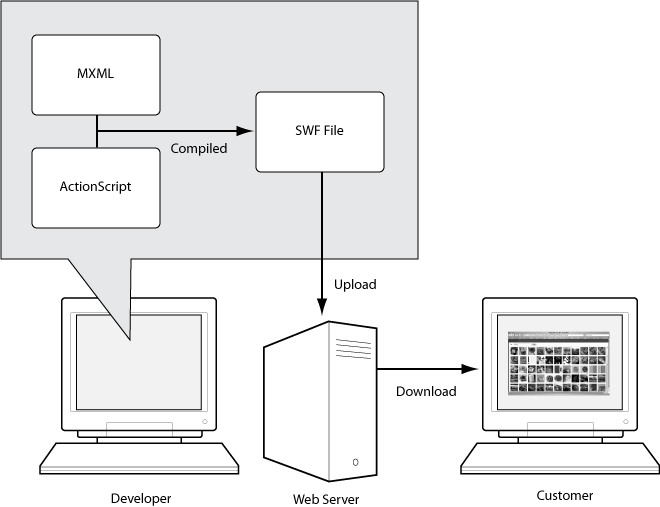
\includegraphics[width=7cm]{./images/as_to_swf}
\caption{\label{fig:as_to_swf} Proses kompilasi, \textit{deploy} dan akses aplikasi}
\end{center}
\end{figure}

